% !TEX encoding = UTF-8 Unicode
\documentclass[convert={density=300,size=1000x700,outext=.png}]{standalone}
\usepackage{tikz}
% \usepackage[active,tightpage,psfixbb]{preview}
\usepackage{tipa}
% \PreviewEnvironment{pgfpicture}
% \setlength\PreviewBorder{2pt}

\begin{document}
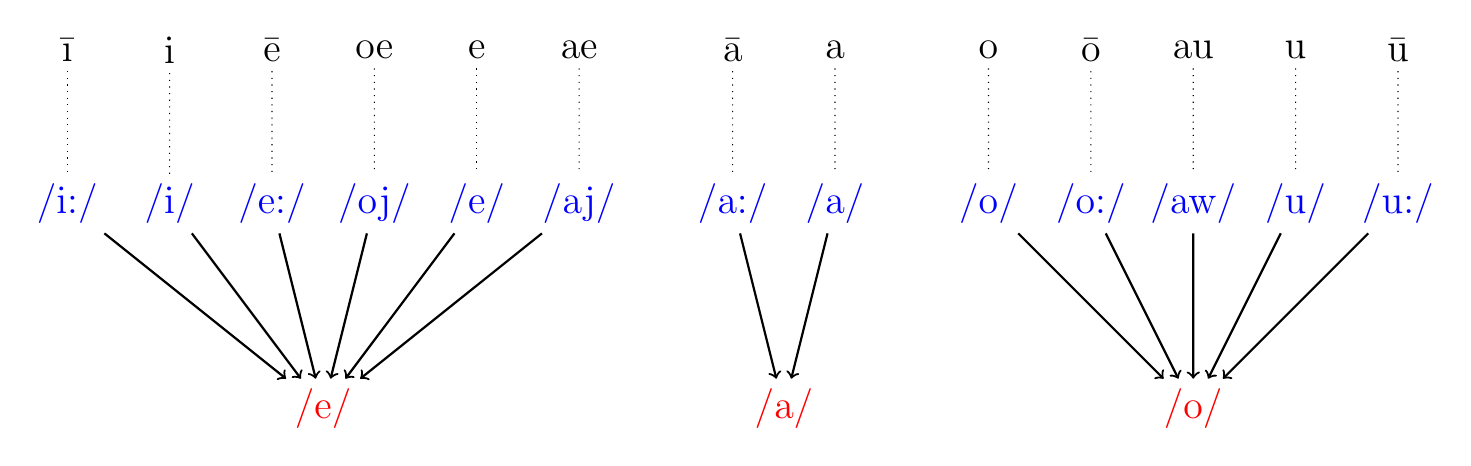
\begin{tikzpicture}[scale=.65]

% graphemes
\node [font=\Large] (a1) at (0,3) {\={\i}};
\node [font=\Large] (a2) at (2,3) {i};
\node [font=\Large] (a3) at (4,3) {\={e}};
\node [font=\Large] (a4) at (6,3) {oe};
\node [font=\Large] (a5) at (8,3) {e};
\node [font=\Large] (a6) at (10,3) {ae};

\node [font=\Large] (a7) at (13,3) {\={a}};
\node [font=\Large] (a8) at (15,3) {a}; 

\node [font=\Large] (a9) at (18,3) {o};
\node [font=\Large] (a10) at (20,3) {\={o}};
\node [font=\Large] (a11) at (22,3) {au};
\node [font=\Large] (a12) at (24,3) {u};
\node [font=\Large] (a13) at (26,3) {\={u}};


% vowels 1
\node [font=\Large,blue] (b1) at (0,0) {\textipa{/i:/}};
\node [font=\Large,blue] (b2) at (2,0) {\textipa{/i/}};
\node [font=\Large,blue] (b3) at (4,0) {\textipa{/e:/}};
\node [font=\Large,blue] (b4) at (6,0) {\textipa{/oj/}};
\node [font=\Large,blue] (b5) at (8,0) {\textipa{/e/}};
\node [font=\Large,blue] (b6) at (10,0) {\textipa{/aj/}};

\node [font=\Large,blue] (b7) at (13,0) {\textipa{/a:/}};
\node [font=\Large,blue] (b8) at (15,0) {\textipa{/a/}}; 

\node [font=\Large,blue] (b9) at (18,0) {\textipa{/o/}};
\node [font=\Large,blue] (b10) at (20,0) {\textipa{/o:/}};
\node [font=\Large,blue] (b11) at (22,0) {\textipa{/aw/}};
\node [font=\Large,blue] (b12) at (24,0) {\textipa{/u/}};
\node [font=\Large,blue] (b13) at (26,0) {\textipa{/u:/}};


% lines 1
\draw [dotted] (a1) -- (b1);
\draw [dotted] (a2) -- (b2);
\draw [dotted] (a3) -- (b3);
\draw [dotted] (a4) -- (b4);
\draw [dotted] (a5) -- (b5);
\draw [dotted] (a6) -- (b6);
\draw [dotted] (a7) -- (b7);
\draw [dotted] (a8) -- (b8);
\draw [dotted] (a9) -- (b9);
\draw [dotted] (a10) -- (b10);
\draw [dotted] (a11) -- (b11);
\draw [dotted] (a12) -- (b12);
\draw [dotted] (a13) -- (b13);



%vowels 2
\node [font=\Large,red] (c1) at (5,-4) {\textipa{/e/}};
\node [font=\Large,red] (c2) at (14,-4) {\textipa{/a/}};
\node [font=\Large,red] (c3) at (22,-4) {\textipa{/o/}};


% lines 2
\draw [->, thick] (b1) -- (c1);
\draw [->, thick] (b2) -- (c1);
\draw [->, thick] (b3) -- (c1);
\draw [->, thick] (b4) -- (c1);
\draw [->, thick] (b5) -- (c1);
\draw [->, thick] (b6) -- (c1);

\draw [->, thick] (b7) -- (c2);
\draw [->, thick] (b8) -- (c2);

\draw [->, thick] (b9) -- (c3);
\draw [->, thick] (b10) -- (c3);
\draw [->, thick] (b11) -- (c3);
\draw [->, thick] (b12) -- (c3);
\draw [->, thick] (b13) -- (c3);


\end{tikzpicture}
\end{document}